\documentclass[12pt]{article}
\usepackage{amsmath}
\usepackage{askmaps}
\usepackage{graphicx}
\usepackage{wrapfig}
\usepackage{booktabs}
\usepackage[letterpaper, margin=1in]{geometry}
\usepackage{fancyhdr}
\usepackage [autostyle, english = american]{csquotes}
\MakeOuterQuote{"}
\renewcommand{\baselinestretch}{1.0}
\newcommand{\objects}[2]{%
  \leavevmode\vbox{\hbox{#1}\nointerlineskip\hbox{#2}}%
}
\title{Lab 3 \\ Combinational MSI Circuits}
\author{Qadis Chaudhry}
\date{March 26, 2021}
\begin{document}
\maketitle
\section*{Experiment 1}
\begin{itemize}
    \item[\textit{i)}]
\end{itemize}
\begin{figure}[h]
    \centering
    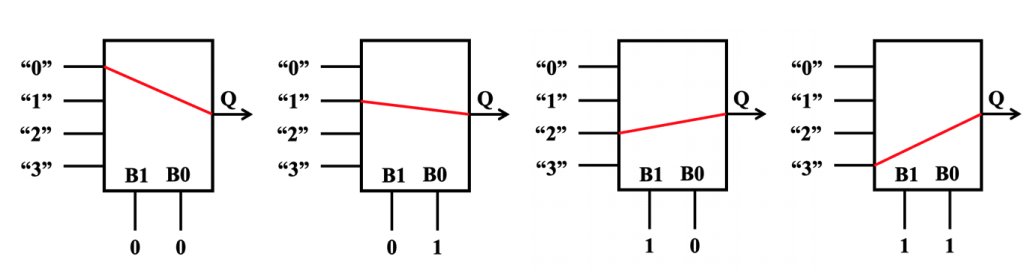
\includegraphics[width=0.9\textwidth]{Experiment 1 Figure 1.png}
    \caption{Switch for 4x1 Multiplexer}
    \label{fig:Experiment-1-part-1-png}
\end{figure}
\par Figure 1 depicts the function of a four-to-one multiplexer and demonstrates
the utility of such a gate. This particular multiplexer takes in six inputs,
four regular inputs and 2 control inputs, and gives one output. The output is
simply one of the inputs, however, the input that is chosen to be the output is
determined by the set of control or "select" data. The multiplexer in essence
serves as a multi-input switch, where regular switches are capable of assuming
two values, a multiplexer can take on a number of values based on the number of
control inputs given. With this knowledge, the truth table describing this
multiplexer can be derived.
\begin{center}
    \begin{tabular}{cc|cccc|c}
        \toprule
        \multicolumn{2}{c}{Select} & \multicolumn{4}{|c|}{Inputs} & Output \\
        \midrule
        B1 & B0 & "3" & "2" & "1" & "0" & Q \\
        \midrule
        0 & 0 & 0 & 0 & 0 & 1 & "0" \\
        0 & 1 & 0 & 0 & 1 & 0 & "1" \\
        1 & 0 & 0 & 1 & 0 & 0 & "2" \\
        1 & 1 & 1 & 0 & 0 & 0 & "3" \\
        \bottomrule
    \end{tabular}
\end{center}
\newpage
\par This truth table makes evident the fact that the output of a multiplexer is
solely dependent on the structure of the select inputs. Since there are 2 select
inputs, all possible combinations of inputs can be defined as, 00, 01, 10, and
11. With this, each of the input values are coupled to one of the select
combinations, which results in the output of the gate,to be one of the four
given inputs. The inputs are denoted by one when they are active as they will
later be the input of an AND gate with the select inputs and the output of this
gate must be one.
\begin{itemize}
    \item[\textit{ii)}]
\end{itemize}
\begin{center}
    \objects
        {\includegraphics[width=0.7\textwidth]{Experiment 1 (AND-OR, 0001)
        2021-03-12 at 2.03.42 PM.png}}
        {\includegraphics[width=0.7\textwidth]{Experiment 1 (AND-OR, 0010)
        2021-03-12 at 2.03.33 PM.png}}
    \objects
        {\includegraphics[width=0.9\textwidth]{Experiment 1 (AND-OR, 0100)
        2021-03-12 at 2.03.25 PM.png}}
        {\includegraphics[width=0.9\textwidth]{Experiment 1 (AND-OR, 1000)
        2021-03-12 at 2.03.15 PM.png}}
\end{center}
\begin{figure}[h]
    \centering
    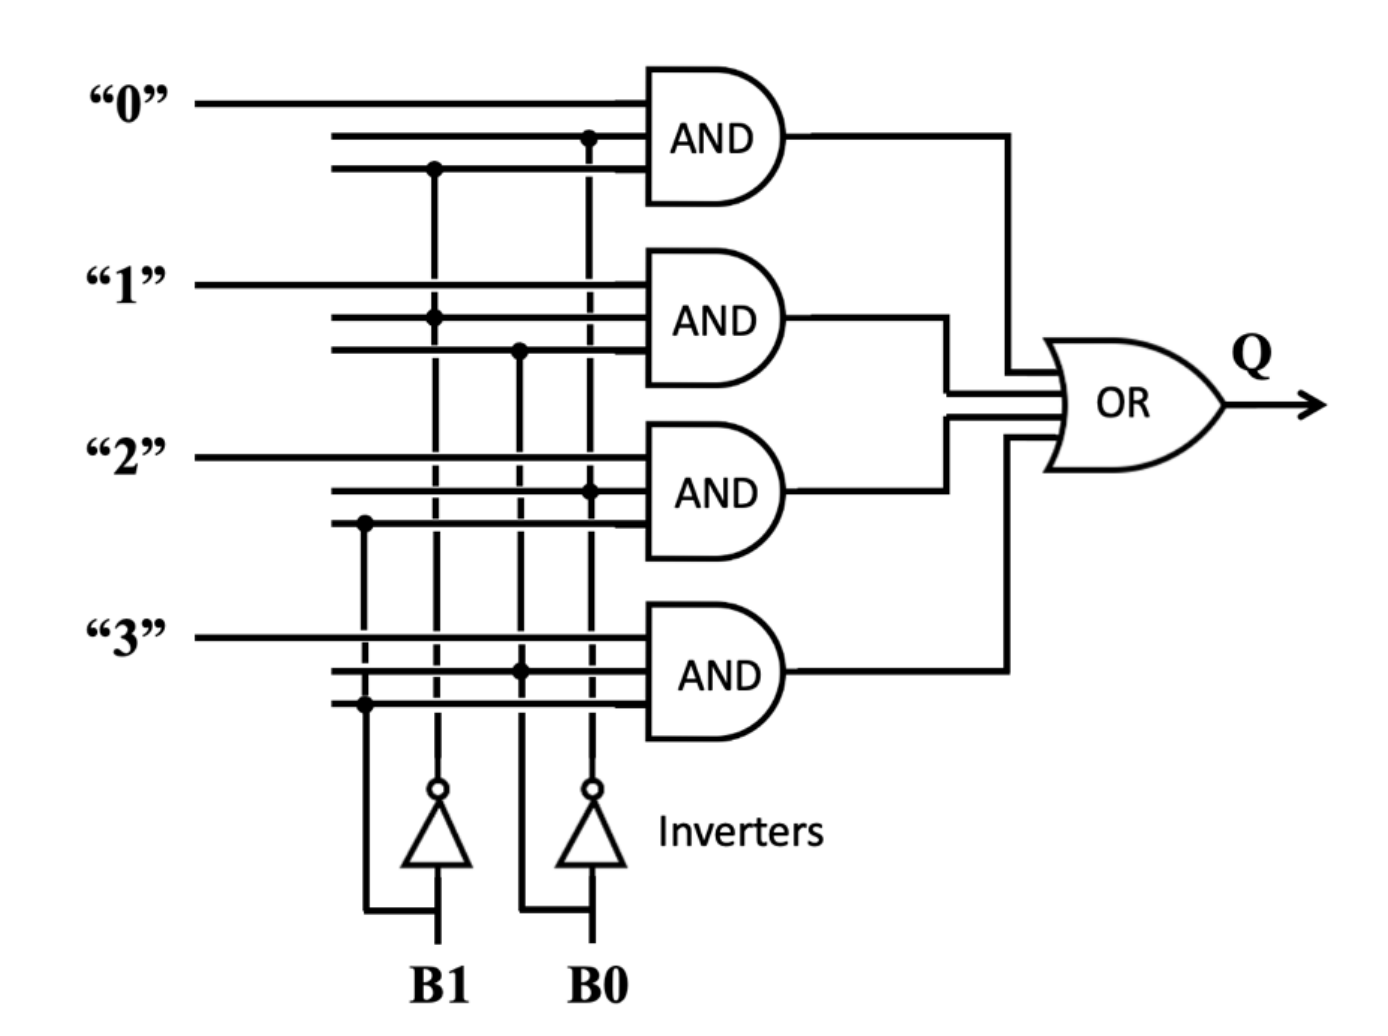
\includegraphics[width=0.8\textwidth]{4x1 Mux AND-OR Circuit Diagram.png}
    \caption{4x1 Mux AND-OR Circuit Diagram}
\end{figure}
\par Shown above is the AND-OR circuit implementation of a four-to-one
multiplexer and its corresponding build in Emona. The select inputs here are
controlled by a binary counter, while the inputs to the gate are held constant
by a switch. This allows for the manual control of the value of the inputs and
therefore, the changes in the output according to its value can be detected. It
also warrants the exemplification of the gate's behavior as, through the
observation of the wave forms, it can be seen that there is only one peak at a
time when the value of one of the inputs is switched to one. This behavior is
apparent since the model itself is based upon the truth table and corresponds
well with it. With four inputs and two select inputs, the select data
systematically assumes a value combination that pertains to one specific switch
input. The four inputs require four AND gates since each of the inputs is ANDed
with a specific combination of the select data.
\par By doing this, the value of the select data is what dictates the output of
the AND gate since the output of the AND gate will be one when the value of all
of its inputs is one. By equating one particular combination to one specific
input, the select data combination will be one and if the input switch
corresponding to that combination also happens to be one, the output of the AND
gate will be one.  Since all of the AND gate outputs are taken as inputs to an
OR gate, the output of the overall gate will exhibit the value of the input
which is set to one.  This setup is what eventually allows for only one of the
AND gates to be active based on the value of the select data and therefore, one
of the inputs is relayed to the output.
\par Another method of implementation of this gate is with NAND gates and can be
done just as efficiently.
\begin{itemize}
    \item[\textit{iii)}]
\end{itemize}
\begin{center}
    \objects
        {\includegraphics[width=0.87\textwidth]{Experiment 1 (NAND-NAND, 0001)
        2021-03-12 at 2.17.41 PM.png}}
        {\includegraphics[width=0.87\textwidth]{Experiment 1 (NAND-NAND, 0010)
        2021-03-12 at 2.17.33 PM.png}}
    \objects
        {\includegraphics[width=0.9\textwidth]{Experiment 1 (NAND-NAND, 0100)
        2021-03-12 at 2.17.25 PM.png}}
        {\includegraphics[width=0.9\textwidth]{Experiment 1 (NAND-NAND, 1000)
        2021-03-12 at 2.17.17 PM.png}}
\end{center}
\begin{figure}[h]
    \centering
    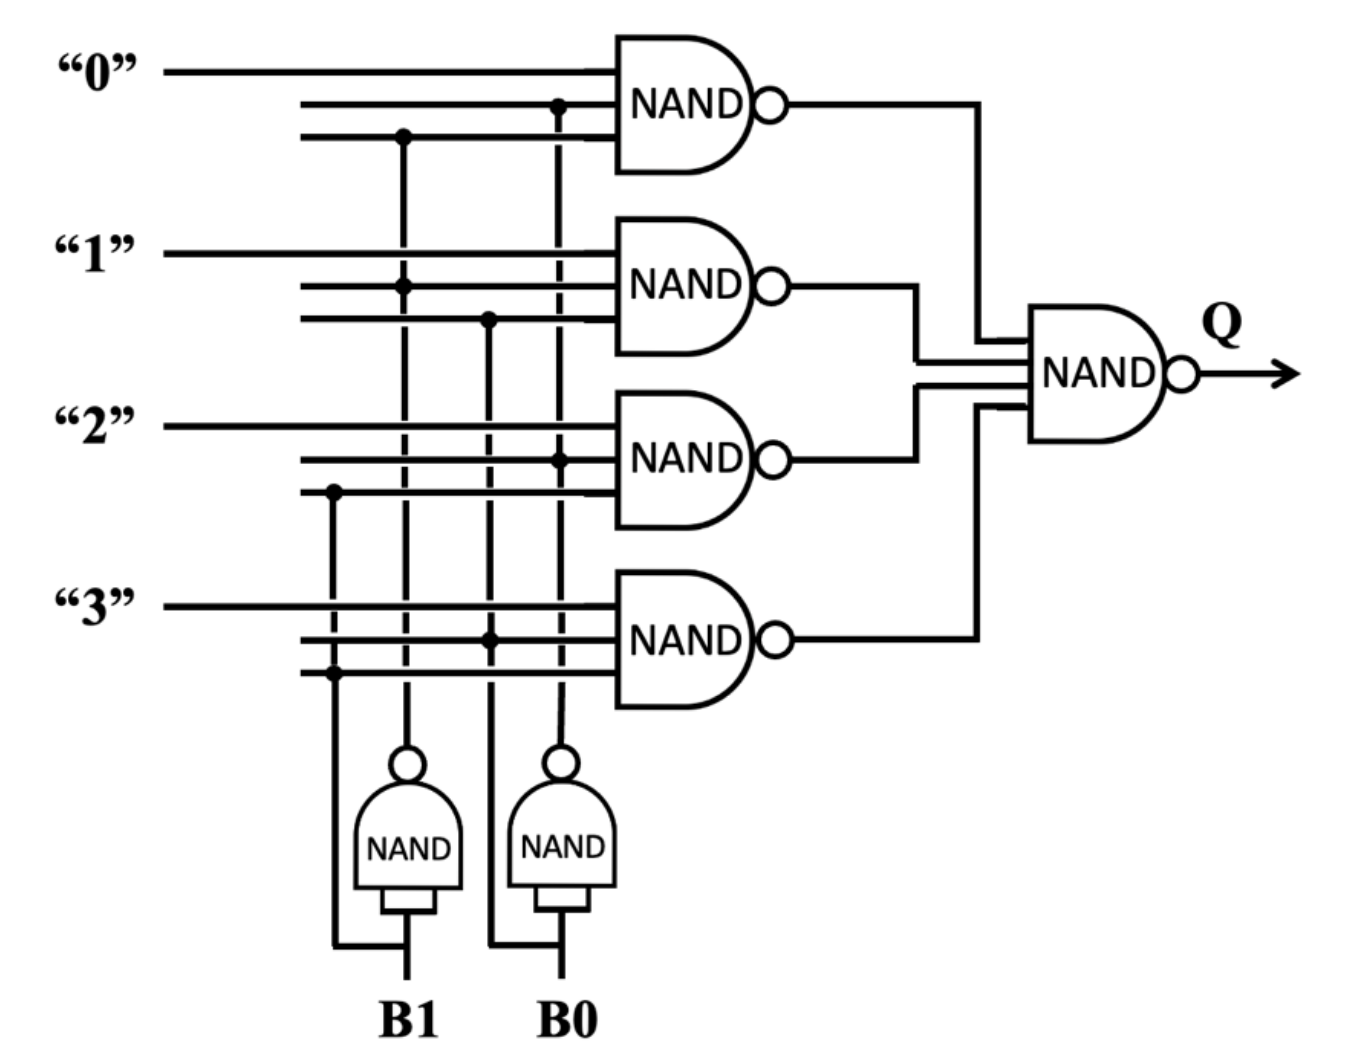
\includegraphics[width=0.8\textwidth]{4x1 Mux NAND-NAND Circuit Diagram.png}
    \caption{4x1 Mux NAND-NAND Circuit Diagram}
\end{figure}
\par It is known that Boolean circuits can be expressed using a select few
combination of gates. The three main implementations are AND-OR, NAND-NAND, and
NOR-NOR. These three two level implementations are able to successfully
describe any Boolean expression and in this case, we have used the typical
AND-OR, sum-of-products, approach, however, we can also implement this gate
using only NAND gates. In the figure above, the NAND-NAND circuit is shown along
with its Emona realization, which consists of the wave forms that will be
compared to the AND-OR model in the future.
\par The reason we are able to create a circuit with only NAND gates has to do
with the fact that NAND gates are able to replicate every other gate, AND, OR,
and NOT, needed for the realization of a circuit. For a NOT gate, or an
inverter, the value that is needing to be inverted is taken as both inputs to
the gate and the output will be the inverted version of that value. This is
because the function of a NAND gate is equivalent to that of an AND gate with an
inverter at its output. By taking the desired value as both inputs, we know that
any value ANDed with itself simply gives back the value, $x \cdot x = x$, and
since the value of this AND operation is then inverted, the value that is
attained from the output of the NAND gate is $x'$. This principle is used for
the inversion of the select data variables, $B0$ and $B1$.
\par Furthermore, we can see how the rest of the circuit resembles the AND-OR
model as well. By splitting the four NAND gates in the middle into AND gates
with an inverter at their output, we can see the resemblance with the other
model in this section of the circuit. Now doing the same with the NAND gate at
the end, the resulting circuit has four AND gates in the middle, followed by
inverters, followed by one AND gate, and finally an inverter at the end. If we
look past the first set of AND gates, the NOT gates can be coupled with the
singular AND gate yielding an AND gate with an inverter at each of its four
inputs. The expression for this gate will take the form $(x'y'z'w')$. Now, using
the DeMorgan's Law, this can be rewritten as, $(x+y+z+w)'$. This expression is
one that describes a common gate, the NOR gate. This shows that the AND gate
with four inverted inputs is equivalent to a four input NOR gate. The final
remaining aspect in this circuit to convert it into the AND-OR form is the
inverter at the end. If we use the same expression for the purpose of
exemplification, by the Law of Double Negation, $((x+y+z+w)')' = x+y+z+w$. This
gives us the final form of the circuit using AND-OR gates, where four AND gates
are present in the middle, with an OR gate providing the output at the end as it
takes the outputs of the AND gates as its input.
\par Now that it has been shown that the two circuit implementations are equal,
it can be said by the same reasoning that they perform the same function. This
implementation is no different from the AND-OR model and therefore, describes
the function of a four-to-one multiplexer in the same manner. The circuit acts
as a multi-input switch where the output is dependent solely on the select data
that is given and from it, the circuit relays one of the inputs to the overall
output in the end.
\par The truth table can be used to verify the function of this circuit as it
was used for the previous one as well. As explained previously, the output of
the function is dependent on the select inputs and the truth table shows that
the value of the output will be one of the inputs, based on the value of the
select inputs. Another method of verification of the circuit is by comparing the
wave forms of the two implementations. Since we saw that the AND-OR
implementation was correspondent with the truth table, we can compare the wave
forms directly and observe their equivalence. It can be seen that both waveforms
are seemingly indistinguishable from one another and for this reason they must
be equivalent. Since they are equivalent, both implementations are equivalent
and since one of them represents the truth table, both of them must be accurate
representations of the four-to-one multiplexer.
\newpage
\begin{itemize}
    \item[\textit{iv)}]
\end{itemize}
\begin{figure}[h]
    \centering
    \includegraphics[width=0.9\textwidth]{Experiment 1 (8x1 Multiplexer
    00000001).png}
\end{figure}
\objects
    {\includegraphics[width=0.5\textwidth]{Experiment 1 (8x1 Multiplexer
    00000010).png}}
    {\includegraphics[width=0.5\textwidth]{Experiment 1 (8x1 Multiplexer
    00000100).png}}
\objects
    {\includegraphics[width=0.5\textwidth]{Experiment 1 (8x1 Multiplexer
    00001000).png}}
    {\includegraphics[width=0.5\textwidth]{Experiment 1 (8x1 Multiplexer
    00010000).png}}
\begin{center}
    \objects
        {\includegraphics[width=0.75\textwidth]{Experiment 1 (8x1 Multiplexer
        00100000).png}}
        {\includegraphics[width=0.75\textwidth]{Experiment 1 (8x1 Multiplexer
        01000000).png}}
        {\includegraphics[width=0.75\textwidth]{Experiment 1 (8x1 Multiplexer
        10000000).png}}
\end{center}
\par Shown above is the realization of an eight-to-one multiplexer using AND,
NAND, NOT, and OR gates, with the use of the Emona system. The first image shows
the circuit implementation of the multiplexer with the values of the input being
set to 00000001. The rest of the images are the waveforms obtained by setting
the next corresponding input equal to 1. It can be seen that the waveforms of
this multiplexer are similar to those of the four-to-one multiplexer, the only
difference being, this time there are more inputs and select inputs. Each of the
waveforms seems to display the same behavior as seen with the four-to-one
multiplexer, there is one peak for each input change. As explained previously,
the fundamental goal of a multiplexer is to function as a multi-input switch.
For the attainment of that goal, a simple template is followed where, the inputs
of the select data are coupled with a specific switch input within an AND gate,
and these AND gates are then relayed as the inputs of an OR gate. This functions
to allow the input that is selected based on the control input combination to be
the input that is active at the output, otherwise, all other inputs are
inactive.
\par Extrapolating from the implementation of the four-to-one multiplexer, in
order to realize the eight-to-one multiplexer, we would require eight quadruple
input AND gates and one eight input OR gate. Not only is this very inefficient,
the Emona system does not have the required resources needed for this type of
implementation.  This would be the same case for a NAND-NAND implementation
which means, another method of implementation must be devised. For this
particular scenario, the concept of cascading multiplexers was utilized. Since
an eight-to-one multiplexer has eight inputs and three select inputs, we can use
four two-to-one multiplexers along with one four-to-one multiplexer in order to
simulate an eight-to-one multiplexer. The four two-to-one multiplexers will
cover the eight regular inputs as well as one of the select inputs, as each two
to one multiplexer has two inputs and one select input. The output of these can
then be taken as the input of the four-to-one multiplexer which has two select
inputs, thereby covering all eight regular inputs as well as the three select
inputs.
\par Despite this approach, we still lack the required materials since in order
to implement the four two-to-one multiplexers, we need eight dual input AND
gates. This can be worked around as since we do have access to dual input NAND
gates, and since we know the function of a NAND gate is equivalent to the
inversion of the output of an AND gate, simply inverting the output of a NAND
gate will yeild a functionally equivalent AND gate. With this in mind, we are
able to use the six available dual input AND gates and two dual input NAND
gates to achieve the eight needed AND gates for the implementation. The outputs
of these AND gates are taken as the input of four corresponding OR gates to
complete the creation of the two-to-one multiplexers. For the four-to-one
multiplexer, we can implement it as we did before, with the use of four triple
input AND gates and a quadruple input OR gate. Taking the outputs of the OR
gates as the input of the AND gates for the four-to-one multiplexer, we can feed
the outputs of these four AND gates to the quadruple input OR gate. This will
yield the final output, a functionally identical eight-to-one multiplexer.
\par To verify the validity of our creation, we can compare the output of the
waveforms to the truth table of an eight-to-one multiplexer.
\begin{center}
    \begin{tabular}{ccc|cccccccc|c}
        \toprule
        \multicolumn{3}{c}{Select} & \multicolumn{8}{|c|}{Inputs} & Output \\
        \midrule
        B2 & B1 & B0 & "7" & "6" & "5" & "4" &"3" & "2" & "1" & "0" & Q \\
        \midrule
        0 & 0 & 0 & 0 & 0 & 0 & 0 & 0 & 0 & 0 & 1 & "0" \\
        0 & 0 & 1 & 0 & 0 & 0 & 0 & 0 & 0 & 1 & 0 & "1" \\
        0 & 1 & 0 & 0 & 0 & 0 & 0 & 0 & 1 & 0 & 0 & "2" \\
        0 & 1 & 1 & 0 & 0 & 0 & 0 & 1 & 0 & 0 & 0 & "3" \\
        1 & 0 & 0 & 0 & 0 & 0 & 1 & 0 & 0 & 0 & 0 & "4" \\
        1 & 0 & 1 & 0 & 0 & 1 & 0 & 0 & 0 & 0 & 0 & "5" \\
        1 & 1 & 0 & 0 & 1 & 0 & 0 & 0 & 0 & 0 & 0 & "6" \\
        1 & 1 & 1 & 1 & 0 & 0 & 0 & 0 & 0 & 0 & 0 & "7" \\
        \bottomrule
    \end{tabular}
\end{center}
\par This is the truth table for an eight-to-one multiplexer and it can be seen
that it is just an extrapolation of the truth table made for the four-to-one
multiplexer in the beginning of the experiment. The difference here is that
there are more inputs and therefore more combinations for the select input data.
The output here will be one of the eight possible inputs given to the system.
With this table, we can verify the waveforms granted by the Emona system.
\par The waveforms are seen to be similar to those of the four input multiplexer
as well, with the flip of one of the switches at a time, there is one peak that
is created in the graph. In this case, for each of the eight input switches,
there is one peak created which shows that the model is working as intended. The
truth table shows that there should only be one input chosen as the output and
it can be seen in the waveforms that whichever switch is chosen to be active
high, is relayed as the output of the gate. This choice is based upon the select
input data.
\section*{Experiment 2}
\begin{figure}[h]
    \centering
    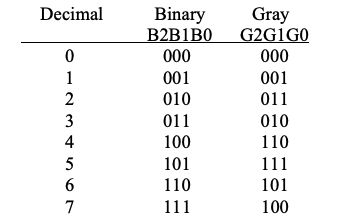
\includegraphics[width=0.6\textwidth]{Binary to Gray.png}
    \caption{Binary to Gray conversion table}
\end{figure}
\begin{figure}[h]
    \begin{minipage}{.55\textwidth}
        \centering
        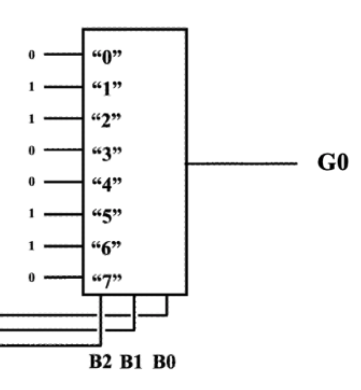
\includegraphics[width=0.9\textwidth]{Encoder for G0.png}
    \end{minipage}
    \begin{minipage}{.5\textwidth}
        \centering
        \objects
            {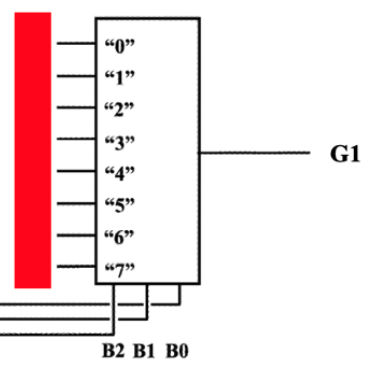
\includegraphics[width=0.5\textwidth]{Encoder for G1.png}}
            {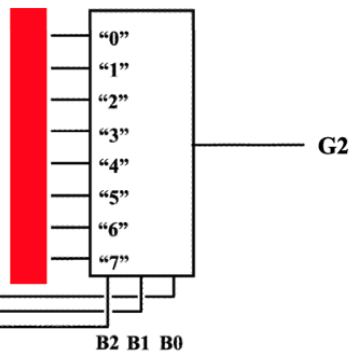
\includegraphics[width=0.5\textwidth]{Encoder for G2.png}}
    \end{minipage}
    \caption{Encoders for G0, G1 and G2}
\end{figure}
\begin{itemize}
    \item[\textit{i)}]
\end{itemize}
\par The figure above shows the encoders for the bits of the Gray Code. The
inputs must be determined based on the conversion of binary to this code and the
reason for this is the fact that the binary bits are being used as the control
inputs for the multiplexers. The value of the inputs for $G0$ have been given to
us and it can be seen that they directly correspond to the conversion of the
last digit from binary to Gray. This suggests that the values of $G1$ and $G2$
also scale in this way. This means that the numbers under the orange rectangle
for the encoder of $G1$ will be, 0,0,1,1,1,1,0,0. With this same ideology, we
can define the inputs for the encoder of $G2$ as well, 0,0,0,0,1,1,1,1. This
way, depending on the value of the binary digit that is being coded, the correct
values for each bit, $G0$, $G1$, and $G2$ will be attained from each of the
respective multiplexers.
\begin{itemize}
    \item[\textit{ii)}]
\end{itemize}
\par Using the values in the conversion table, we can employ the use of Karnaugh
Maps in order to create expressions for each of the binary bits needed to be
converted from the Gray code. Since there are three inputs in this case, $G0$,
$G1$, and $G2$, we will need a eight cell Karnaugh Map with the inputs being the
Gray bits and the logic functions being the values of the binary bits. To prove
that the bit $B1$ is the XOR of the Gray bits $G1$ and $G2$, we will use this
technique of using the Karnaugh Map. Here, $G0$, $G1$, and $G2$ will be given by
the letters A, B, and C, respectively.
\begin{center}
    \askmapiiialt{}{ACB}{F}{01100110}{}
\end{center}
\par This is the map for the bit $B1$ and it can be seen that within this map,
there are two distinct groups that can be defined, cells 1 and 5, and cells 2
and 6. Once these are grouped, an expression for them can be determined and from
there, the rest of the bits must be defined in order to realize a design for the
decoder.
\begin{center}
    \askmapiiialt{}{ACB}{F}{01100110}{%
        \put(1.0,2.5){\oval(1.8,0.8)}%
        \put(1.0,0.5){\oval(1.8,0.8)}%
    }
\end{center}
\par These are the two prime implicants that can be formed from this map. The
top group, cells 1 and 5, can be defined as, $G2'G1$, and the other group can be
defined as $G2G1'$. This gives the resulting function for the map, and the
expression for the bit $B1$, as \\ $B1 = G2'G1 + G2G1'$. Recognizing this function
as being the definition of the XOR gate, we can rewrite the expression as
simply, $B1 = G1 \oplus G2$.
\begin{center}
    \askmapiiialt{}{ACB}{F}{01101001}{}
\end{center}
\par For the bit $B0$ we can use this map shown above. This map is of the same
variables, the bits of the Gray code, and it is now defined to describe the
expression of the bit $B0$. With this map, there are a few groups that can be
defined, $G2'G1'G0$, $G2'G1G0'$, $G2G1'G0'$, and $G2G1G0$. With this, the
function for the bit $B0$ can be written as $B0 = G2'G1'G0 + G2'G1G0' + G2G1'G0'
+ G2G1G0$, however, this can be simplified down much further. Factoring out the
$G2'$ as well as the $G2$ we get, $G2'(G1'G0+G1G0') + G2(G1'G0'+G1G0)$. Once
again, the expression for the XOR is present meaning those terms can be written
as the inputs of an XOR gate: $ G2'(G1 \oplus G0) + G2(G1 \oplus G0)'$. Finally,
this can be written as simply the input of one triple input XOR gate giving the
final expression, $B0 = G0 \oplus G1 \oplus G2$.
\begin{center}
    \askmapiiialt{}{ACB}{F}{00110011}{}
\end{center}
\par The last bit that needs to be defined is bit $B2$, and a Karnaugh Map can
be used for this as well. The one shown above is defined for the bit $B2$ and it
can be seen that one group of 4 cells, cells 2, 3, 6 and 7, is able to be formed.
\begin{center}
    \askmapiiialt{}{ACB}{F}{00110011}{%
        \put(1.0,1.0){\oval(1.8,1.8)}%
    }
\end{center}
\par With this, the expression for this bit can be defined. This group can be
defined simply as $G2$ meaning, that the bit $B2$ is only dependent on the value
of $G2$.
\par Using all of this information, $B0 = G0 \oplus G1 \oplus G2$, $B1 = G2'G1 +
G2G1'$, $B2 = G2$ and  we are finally able to construct the design of the
decoder.
\newpage
\begin{itemize}
    \item[\textit{iii)}]
\end{itemize}
\par Using the findings form the previous section, we can implement the circuit
using the Emona system. The simplicity in this case is that the only gate
necessary is the XOR gate, the rest of the materials are merely just the inputs,
the Gray and binary counters.
\begin{figure}[h]
    \centering
    \includegraphics[width=0.8\textwidth]{Experiment 2 (Decoder) 2021-03-12 at
    3.04.52 PM.png}
    \caption{Gray to Binary Decoder}
\end{figure}
\par Here it can be seen that there are three outputs that are being monitored
by the channels. These three outputs are the binary bits that are being
converted from the Gray code counter. There are three XOR gates that are in use
and two of them are outputs while one is the input to another gate. This is
because there are only dual input XOR gates available in Emona and therefore a
workaround must be devised. In this case it was as simple as taking the XOR
output of two of the variables and using that as the input to another XOR with
the third variable. This leads to the expression of the binary bit $B0$. The bit
$B1$ is able to be sufficed with the use of one gate and the value of the bit
$B2$ is the simplest as it is a direct output in this case.
\par Looking at the waveforms it can be seen from one period that the decoder is
working as the binary code is seen to be accurate across the readings. The value
of the Gray code is not monitored however, by looking at the binary output of
the code, it is evident that the code is being converted from Gray to binary. If
the zero and one values are placed on the binary outputs within the waveform, it
can be seen that the outputs correspond with the table given for the conversion
of the code. This tells us that the decoder is working.
\end{document}
